\documentclass[12pt, a4paper]{article}

% ==============================================================================
% PACKAGES
% ==============================================================================

\usepackage[utf8]{inputenc}
\usepackage[margin=1in]{geometry}
\usepackage{setspace}
\onehalfspacing

\usepackage{amsmath, amssymb, amsfonts}
\usepackage{graphicx}
\usepackage{booktabs}
\usepackage{tocloft}
\usepackage{array}
\usepackage{multirow}
\usepackage{listings}
\usepackage{xcolor}
\usepackage{hyperref}
\usepackage{fancyhdr}
\usepackage{tabularx}
\usepackage{caption}
\usepackage{subcaption}
\usepackage{enumitem}
\usepackage{tikz}
\usepackage{pgfplots}
\pgfplotsset{compat=1.18}

\usetikzlibrary{positioning,arrows.meta,calc,shapes.geometric}

% ==============================================================================
% HYPERREF SETUP
% ==============================================================================

\hypersetup{
    colorlinks=true,
    linkcolor=blue,
    citecolor=blue,
    urlcolor=cyan,
    pdftitle={Design and Implementation of a Real-Time Chat System},
    pdfauthor={Le Huy Hoang}
}

% ==============================================================================
% CODE LISTINGS CONFIGURATION
% ==============================================================================

\definecolor{codegray}{rgb}{0.5,0.5,0.5}
\definecolor{codepurple}{rgb}{0.58,0,0.82}
\definecolor{backcolour}{rgb}{0.96,0.96,0.96}
\definecolor{codeblue}{rgb}{0.13,0.29,0.53}

\lstdefinestyle{codeStyle}{
    backgroundcolor=\color{backcolour},
    commentstyle=\color{codegray}\itshape,
    keywordstyle=\color{codeblue}\bfseries,
    numberstyle=\tiny\color{codegray},
    stringstyle=\color{codepurple},
    basicstyle=\ttfamily\footnotesize,
    breakatwhitespace=false,
    breaklines=true,
    captionpos=b,
    keepspaces=true,
    numbers=left,
    numbersep=8pt,
    showspaces=false,
    showstringspaces=false,
    showtabs=false,
    tabsize=2
}

% ------------------------------------------------------------------------------
% NGINX LANGUAGE DEFINITION
% ------------------------------------------------------------------------------

\lstdefinelanguage{nginx}{
    keywords={
        server,
        listen,
        server_name,
        return,
        ssl_certificate,
        ssl_certificate_key,
        root,
        index,
        location,
        try_files,
        proxy_pass,
        proxy_http_version,
        proxy_set_header
    },
    sensitive=true,
    comment=[l]{\#},
    morestring=[b]"
}

\lstset{style=codeStyle}

% ==============================================================================
% HEADER & FOOTER
% ==============================================================================

\pagestyle{fancy}
\fancyhf{}

\rhead{Le Huy Hoang (23BI14172)}
\lhead{Nextalk Real-Time Chat System}
\rfoot{Page \thepage}

% ==============================================================================
% SECTION NUMBERING AND TABLE OF CONTENTS
% ==============================================================================

% Main chapters:
% I/ INTRODUCTION
% II/ OBJECTIVES
% III/ MATERIALS AND METHODS
% IV/ RESULTS AND DISCUSSION
% V/ CONCLUSION & PERSPECTIVE

\renewcommand{\thesection}{\Roman{section}/}

% Subsections:
% III/1 Development Environment and Technology Stack
% III/2 System Architecture and Development Approach

\renewcommand{\thesubsection}{\thesection\arabic{subsection}}

% Subsubsections:
% III/3.1 REST API Implementation
% III/3.2 Real-Time Communication Implementation

\renewcommand{\thesubsubsection}{\thesubsection.\arabic{subsubsection}}

% ------------------------------------------------------------------------------
% TABLE OF CONTENTS NUMBER WIDTH
% ------------------------------------------------------------------------------

\setlength{\cftsecnumwidth}{3.5em}
\setlength{\cftsubsecnumwidth}{4.8em}
\setlength{\cftsubsubsecnumwidth}{5.8em}

% Add a small gap between the number and the title
\renewcommand{\cftsecaftersnum}{\hspace{0.5em}}
\renewcommand{\cftsubsecaftersnum}{\hspace{0.5em}}
\renewcommand{\cftsubsubsecaftersnum}{\hspace{0.5em}}

% ==============================================================================
% DOCUMENT BEGIN
% ==============================================================================

\begin{document}

% ==============================================================================
% TITLE PAGE
% ==============================================================================

\begin{titlepage}
    \centering

    % UNIVERSITY
    {\large UNIVERSITY OF SCIENCE AND TECHNOLOGY OF HANOI}\\[0.2cm]

    {\large \textbf{DEPARTMENT OF INFORMATION AND COMMUNICATION TECHNOLOGY}}

    \vspace{1.3cm}

    % USTH LOGO
    \includegraphics[width=0.34\textwidth]{logo-usth-.png}

    \vspace{1.4cm}

    % THESIS TYPE
    {\fontsize{25}{30}\selectfont \textbf{BACHELOR THESIS}}

    \vspace{0.8cm}

    {\large By}

    \vspace{0.3cm}

    {\large \textbf{Le Huy Hoang}}

    \vspace{1.0cm}

    {\large Title:}

    \vspace{0.4cm}

    \begin{minipage}{0.80\textwidth}
        \centering
        {\fontsize{17}{22}\selectfont
        \textbf{Design and Implementation of a Real-Time Chat System}}
    \end{minipage}

    \vfill

    % SUPERVISOR INFORMATION
    \begin{center}
    \begin{tabular}{ll}
        \textbf{External Supervisor:} & Dr. Dau Thanh Van Chuong \\[0.3cm]
        \textbf{Internal Supervisor:} & Dr. Le Nhu Chu Hiep
    \end{tabular}
    \end{center}

    \vfill

    % DATE
    {\large \textbf{Hanoi, August 2026}}

\end{titlepage}

% ==============================================================================
% SUPERVISOR SIGNATURE
% ==============================================================================

\newpage
\thispagestyle{empty}

\vspace*{1.5cm}

\begin{center}
    To whom it may concern,
\end{center}

\vspace{0.8cm}

I, Dau Thanh Van Chuong, certify that the
thesis report of Mr. Le Huy Hoang is qualified to be presented in the Internship
July 2025--2026.

\vspace{3cm}

\begin{flushright}
    Hanoi, \underline{\hspace{2.5cm}}\\[0.8cm]
    \textbf{Supervisor's signature}
\end{flushright}

\newpage

% ==============================================================================
% CONTENTS AND PAGE NUMBERING
% ==============================================================================

\clearpage

% Start Arabic page numbering from the Contents page
\pagenumbering{arabic}
\setcounter{page}{1}

\tableofcontents

\newpage

% ==============================================================================
% ACKNOWLEDGMENTS
% ==============================================================================

\section*{ACKNOWLEDGMENTS}
\addcontentsline{toc}{section}{ACKNOWLEDGMENTS}

I would like to express my deepest appreciation to my supervisor, Dr. Dau Thanh Van Chuong, for their invaluable guidance, continuous support, and patience throughout
this project. Their insights into algorithmic complexity and software architecture
were instrumental in shaping the final outcome of this research.

I also extend my gratitude to the Department of Information and Communication
Technology at the University of Science and Technology of Hanoi for providing a
rigorous academic environment that fostered my technical skills. Finally, I would
like to thank my family and friends for their encouragement during the intensive
development and writing phases of this thesis.

I hope that my work will make a small contribution to the development and
application of information technology in the field of online communication.

\newpage

% ==============================================================================
% LIST OF ABBREVIATIONS
% ==============================================================================

\section*{LIST OF ABBREVIATIONS}
\addcontentsline{toc}{section}{LIST OF ABBREVIATIONS}

\begin{center}
\begin{tabular}{p{3cm} p{10cm}}
\toprule
\textbf{Abbreviation} & \textbf{Meaning} \\
\midrule
API & Application Programming Interface \\
CORS & Cross-Origin Resource Sharing \\
CSS & Cascading Style Sheets \\
E2EE & End-to-End Encryption \\
HTTP & Hypertext Transfer Protocol \\
IM & Instant Messaging \\
JWT & JSON Web Token \\
NGINX & Engine X web server and reverse proxy \\
ORM & Object-Relational Mapping \\
REST & Representational State Transfer \\
SSE & Server-Sent Events \\
SPA & Single-Page Application \\
SQL & Structured Query Language \\
TCP & Transmission Control Protocol \\
TLS & Transport Layer Security \\
UUID & Universally Unique Identifier \\
WSS & WebSocket Secure \\
\bottomrule
\end{tabular}
\end{center}

\newpage

% ==============================================================================
% LIST OF TABLES
% ==============================================================================

\section*{LIST OF TABLES}
\addcontentsline{toc}{section}{LIST OF TABLES}

\listoftables

\newpage

% ==============================================================================
% LIST OF FIGURES
% ==============================================================================

\section*{LIST OF FIGURES}
\addcontentsline{toc}{section}{LIST OF FIGURES}

\listoffigures

\newpage

% ==============================================================================
% ABSTRACT
% ==============================================================================
\section*{ABSTRACT}
\addcontentsline{toc}{section}{ABSTRACT}

In today's digital environment, instant messaging has become an important form of online communication. This thesis presents the design, implementation, and evaluation of \textbf{Nextalk}, a web-based real-time chat and social interaction system.

The backend is developed using Node.js, Express.js, and TypeScript, with Socket.io for real-time communication and REST APIs for conventional client-server operations. Data is managed using Prisma ORM with a MySQL relational database. Security mechanisms include JSON Web Tokens (JWT), Bcrypt password hashing, and Google OAuth 2.0. The system supports user discovery, private messaging, social posts, likes, nested comments, and real-time notifications.

The frontend is implemented as a responsive Single-Page Application using Vite, TypeScript, HTML5, and CSS3. The system was evaluated through functional testing and selected performance measurements focusing on message delivery, database operations, authentication, and the correctness of the main implemented features.

\vspace{0.5cm}
\noindent \textbf{Keywords:} Real-time Communication, Socket.io, Node.js, TypeScript, MySQL, JWT Authentication.

\newpage

% ==============================================================================
% I/ INTRODUCTION
% ==============================================================================

\section{INTRODUCTION}

\subsection{Global Context and Problem Statement}

Instant messaging (IM) has become an essential part of modern digital communication, playing an increasingly important role in both personal and professional environments. The rapid development of Internet technologies and the widespread adoption of smartphones and web applications have significantly changed the way people communicate, creating a growing demand for fast, convenient, and real-time communication services. Modern messaging platforms are expected not only to deliver messages instantly but also to provide a reliable and responsive user experience across different devices and network conditions.

To meet these requirements, real-time communication has become a fundamental aspect of modern web-based messaging systems. Unlike conventional approaches that rely on repeated client requests to retrieve new information, real-time communication technologies allow data to be delivered from the server to connected clients as soon as events occur. Among these technologies, the WebSocket Protocol (RFC 6455) provides a standardized mechanism for establishing persistent, full-duplex communication between clients and servers over a single TCP connection. This enables efficient bidirectional data exchange with low latency and reduced communication overhead, making WebSocket particularly suitable for applications such as instant messaging, online collaboration, notifications, and other real-time services.

However, developing a robust real-time communication system involves several critical software engineering challenges:

\begin{enumerate}
    \item \textbf{Low-Latency Bidirectional Messaging:} Maintaining active connections between clients so that messages can be delivered promptly while preserving the state of the conversation.

    \item \textbf{User Identity and Security:} Protecting user credentials, supporting authentication through Google OAuth, and validating authenticated requests for REST API operations and real-time communication.

    \item \textbf{User Discovery and Friend Networks:} Providing an intuitive way to find users without exposing raw database primary keys, using unique 6-digit identifiers and UUID-based invitation codes.

    \item \textbf{Data Persistence and Integrity:} Storing conversation histories, media references, user profiles, social posts, likes, comments, and notifications while maintaining relationships between related data.

    \item \textbf{System Maintainability:} Structuring the codebase using TypeScript and Prisma ORM to provide clearer data structures and simplify further development and maintenance.
\end{enumerate}


\subsection{Scientific Background and Literature Review}

Real-time web applications require continuous and responsive data exchange between the server and connected clients. Traditional Hypertext Transfer Protocol (HTTP/1.1) follows a stateless, client-initiated request-response model, where the client normally initiates communication~\cite{rfc7230}. Several techniques have therefore been developed to improve the delivery of time-sensitive information in web applications, including HTTP Short Polling, HTTP Long Polling, Server-Sent Events (SSE), and WebSocket.

\subsubsection{HTTP Short Polling}

HTTP Short Polling is a simple technique in which the client periodically sends HTTP requests to the server to check whether new data is available. If new information exists, the server returns it; otherwise, an empty or unchanged response is returned.

The main advantage of Short Polling is its simplicity, as it can be implemented using standard HTTP requests without requiring a persistent connection or specialized real-time protocol. However, it can generate many unnecessary requests when no new data is available. A shorter polling interval can reduce the waiting time before new data is detected, but it also increases the number of requests generated by the client. Therefore, Short Polling is less suitable for applications requiring frequent and responsive communication.

\subsubsection{HTTP Long Polling}

HTTP Long Polling improves upon Short Polling by keeping the client's HTTP request open on the server until new data becomes available or a timeout is reached~\cite{rfc6202}. Upon receiving a request, the server delays its response until an event occurs or the request reaches its timeout. Once the data is delivered, the HTTP response is completed, and the client issues a new HTTP request to maintain continuous communication.

Although Long Polling reduces the number of unnecessary empty responses compared with Short Polling, it still relies on HTTP request-response communication and requires a new request after each response. Consequently, HTTP headers and request-processing overhead are incurred repeatedly. Under high-frequency messaging conditions, this can increase server load and network overhead compared with persistent real-time communication mechanisms such as WebSocket.

\subsubsection{Server-Sent Events (SSE)}

Server-Sent Events (SSE) provide a standardized mechanism for establishing a persistent, unidirectional HTTP connection through which a server can continuously send event data to a client using the \texttt{text/event-stream} media type~\cite{w3c_sse}.

SSE operates over standard HTTP and provides built-in mechanisms for event identification and automatic reconnection, allowing clients to resume communication when a connection is interrupted. Since SSE uses HTTP, it can also work with existing HTTP infrastructure, including proxies and other network intermediaries.

However, communication flows exclusively from the server to the client. For client-to-server operations, such as sending a chat message or transmitting a typing indicator, the client must use a separate mechanism, typically an HTTP \texttt{POST} request. This makes SSE less suitable for applications requiring frequent bidirectional communication, such as real-time chat systems.

\subsubsection{The WebSocket Protocol (RFC 6455)}

Standardized by the IETF in 2011, \textbf{WebSocket (RFC 6455)} provides a standardized mechanism for establishing persistent, full-duplex communication between a client and a server over a single TCP connection~\cite{rfc6455}.

A WebSocket connection is initially established through an HTTP/1.1 request containing specific upgrade headers. The client requests an upgrade from HTTP to the WebSocket protocol:

\begin{lstlisting}[caption={WebSocket Client Upgrade Request}]
GET /chat HTTP/1.1
Host: server.example.com
Upgrade: websocket
Connection: Upgrade
Sec-WebSocket-Key: dGhlIHNhbXBsZSBub25jZQ==
Sec-WebSocket-Version: 13
\end{lstlisting}

The server validates the request and generates the \texttt{Sec-WebSocket-Accept} value by concatenating the \texttt{Sec-WebSocket-Key} with the WebSocket Globally Unique Identifier (GUID) \texttt{258EAFA5-E914-47DA-95CA-C5AB0DC85B11}, computing the SHA-1 hash of the resulting string, and encoding the hash using Base64. The server then responds with HTTP status code \texttt{101 Switching Protocols}:

\begin{lstlisting}[caption={WebSocket Server Upgrade Response}]
HTTP/1.1 101 Switching Protocols
Upgrade: websocket
Connection: Upgrade
Sec-WebSocket-Accept: s3pPLMBiTxaQ9kYGzzhZRbK+xOo=
\end{lstlisting}

After the handshake is successfully completed, the underlying TCP connection remains open and is used for bidirectional communication through WebSocket frames rather than conventional HTTP request-response messages~\cite{rfc6455}.

WebSocket data frames are encoded according to RFC 6455 Section 5.2. Compared with repeated HTTP request headers, WebSocket uses a lightweight frame structure after the initial connection has been established. The minimum framing overhead for an unmasked server-to-client frame with a payload of up to 125 bytes is 2 bytes, while a masked client-to-server frame with a 64-bit extended payload length requires up to 14 bytes. This persistent communication model makes WebSocket suitable for real-time bidirectional applications such as Nextalk.


\subsection{Motivation and Main Questions}

The development of a real-time chat system provides an opportunity to explore the practical implementation of modern web communication technologies while addressing the fundamental requirements of responsive and reliable online messaging.

Based on the problems described above, this thesis focuses on the integration of real-time communication with authentication, persistent data storage, user discovery, friend management, social interaction, and notification mechanisms within a single web-based system.

The main research questions addressed by this project are:

\begin{enumerate}
    \item How can real-time communication be implemented effectively in a web-based chat system?

    \item How can real-time messaging be integrated with authentication, persistent data storage, user discovery, friend management, social interaction, and notification mechanisms?

    \item How can the implemented system be evaluated in terms of functional correctness and basic real-time communication performance?
\end{enumerate}

% ==============================================================================
% II/ OBJECTIVES
% ==============================================================================
\newpage
\section{OBJECTIVES}

The main goal of this graduation thesis is to design, implement, and
evaluate \textbf{Nextalk}, a web-based real-time chat and social
interaction system. Specific objectives include:

\begin{itemize}
    \item Designing a decoupled client-server architecture using Node.js,
    Express.js, TypeScript, and Vite.

    \item Implementing real-time bidirectional communication using
    Socket.io, with WebSocket transport when available.

    \item Designing a normalized MySQL relational schema managed via
    Prisma ORM.

    \item Establishing user authentication using JWT, Bcrypt, and Google
    OAuth 2.0.

    \item Implementing social networking features, including user profiles,
    friend management through invite codes and IDs, social posts, likes,
    nested comments, and real-time notifications.

    \item Conducting functional and selected performance tests to evaluate
    the correctness and responsiveness of the implemented system.
\end{itemize}

% ==============================================================================
% III/ MATERIALS AND METHODS
% ==============================================================================
\section{MATERIALS AND METHODS}

\subsection{Development Environment and Technology Stack}

The Nextalk system was developed using a combination of local development environments and a cloud-based production environment. The production system was deployed on a Vietnix Cloud Virtual Private Server (VPS) running Ubuntu 22.04 LTS on an x86\_64 architecture. NGINX was used as a reverse proxy to handle incoming HTTP/HTTPS requests and forward them to the application server. Secure communication was provided through TLS/SSL certificates issued by Let's Encrypt. PM2 Process Manager was used to maintain the backend application process and support process recovery. The production database was implemented using MySQL 8.0.

The backend application was developed using Node.js, Express.js v5, and TypeScript. Node.js provided the server-side runtime environment, while Express.js was used to implement HTTP request handling, routing, middleware, and RESTful API endpoints. TypeScript was used to provide static type checking and to maintain consistency between the data structures used by different application components. Prisma ORM was used to define the database schema, manage entity relationships, and provide programmatic access to the MySQL database.

Real-time communication was implemented using Socket.io. The application used event-based communication between connected clients and the backend server, with WebSocket used as the real-time transport when available. Socket.io was used to implement private messaging, typing indicators, connection state updates, and real-time notifications.

Authentication and authorization were implemented using Bcrypt, JSON Web Tokens (JWT), and Google OAuth 2.0. Bcrypt was used to hash passwords before storage, while JWT was used to authenticate protected REST API requests and Socket.io connections. Google OAuth 2.0 was integrated to provide an alternative authentication mechanism using Google accounts. File and image uploads were processed using Multer.

The frontend was implemented as a Single-Page Application using Vite, TypeScript, HTML5, and CSS3. The frontend communicated with the backend through REST APIs for conventional request-response operations and through Socket.io for real-time communication. The user interface was implemented using native web technologies and custom CSS without a third-party frontend UI framework.


\subsection{System Architecture and Development Approach}

The system was designed using a decoupled client-server architecture. The frontend was responsible for user interaction, interface rendering, sending requests, and processing real-time events. The backend handled authentication, application logic, data validation, database operations, file processing, and real-time communication. Persistent application data was stored in the MySQL database through Prisma ORM.

Two communication mechanisms were used according to the type of operation. RESTful HTTP APIs were used for operations following the request-response model, such as authentication, user profile management, user discovery, friendship management, retrieving conversation history, social feed operations, and notification retrieval. Socket.io was used for operations requiring real-time event delivery, including private messages, typing indicators, and live notifications.

The overall implementation structure is summarized in Listing~\ref{lst:system_architecture}. The architecture separates the client interface, backend services, and database layer while allowing REST and real-time communication to share the same authentication and persistence mechanisms.

\begin{lstlisting}[basicstyle=\ttfamily\tiny, caption={Nextalk High-Level Decoupled Architecture Layout}, label={lst:system_architecture}]
+-----------------------------------------------------------------------+
|                            CLIENT SIDE                                |
|  Single Page Application (Vite + TypeScript + HTML5 / CSS3)           |
|                                                                       |
|  [Auth UI]    [Chat Interface]    [Friend List]    [Social Feed UI]   |
+-----------------------------------:-----------------------------------+
                                    |
                  +-----------------+-----------------+
                  |                                   |
           HTTP / REST API                     WebSocket Events
           (JSON Payloads)                    (Socket.io Protocol)
                  |                                   |
+-----------------v-----------------------------------v-----------------+
|                            SERVER SIDE                                |
|  Node.js + Express.js + TypeScript Runtime Engine                     |
|                                                                       |
|  [REST Controllers]   [JWT Auth Middleware]   [Socket.io Manager]    |
|  [Multer File Upload]                         [Connected User Map]    |
+-----------------------------------:-----------------------------------+
                                    |
                            Prisma Client ORM
                                    |
+-----------------------------------v-----------------------------------+
|                           DATABASE LAYER                              |
|  MySQL Relational Database (Users, Messages, Friendships, Posts, etc) |
+-----------------------------------------------------------------------+
\end{lstlisting}


\subsection{Backend Implementation}

The backend was implemented using Node.js, Express.js v5, and TypeScript. Express.js middleware was used to process incoming HTTP requests, perform authentication checks, parse request data, serve uploaded media, and handle application errors. The backend was organized around functional API operations covering authentication, users, friendships, messages, posts, comments, likes, and notifications.

For protected operations, the backend first validated the authentication information before executing the corresponding application logic. Database operations were then performed through Prisma Client, and the resulting data was returned to the frontend through HTTP responses or delivered to connected clients through Socket.io events.

\subsubsection{REST API Implementation}

RESTful APIs were implemented using HTTP methods corresponding to the operations performed by the application. Public endpoints were provided for registration and login, while protected endpoints required authentication. The API supported user profile management, user discovery, friendship operations, conversation history retrieval, file upload, social posts, comments, likes, and notifications.

The main REST API operations implemented in Nextalk are summarized in Table~\ref{tab:api_spec}. The table specifies the endpoint, HTTP method, authentication requirement, and purpose of each operation.

\begin{table}[htbp]
\centering
\caption{Nextalk RESTful API Specification}
\label{tab:api_spec}
\resizebox{\textwidth}{!}{%
\begin{tabular}{p{5.2cm} p{1.5cm} p{2.2cm} p{7.2cm}}
\toprule
\textbf{Endpoint} & \textbf{Method} & \textbf{Auth} & \textbf{Description} \\
\midrule
\texttt{/api/auth/register} & POST & Public &
Registers a new user with credentials and generates a unique 6-digit User ID. \\

\texttt{/api/auth/login} & POST & Public &
Authenticates credentials using Bcrypt and returns a JWT token. \\

\texttt{/api/auth/google} & POST & Public &
Verifies the Google OAuth token and authenticates or creates the corresponding user account. \\

\texttt{/api/auth/me} & GET & Bearer JWT &
Retrieves the authenticated user's profile information. \\

\texttt{/api/profile} & PUT & Bearer JWT &
Updates the authenticated user's profile information. \\

\texttt{/api/friends/search} & GET & Bearer JWT &
Searches for users using a unique 6-digit User ID or Invite Code. \\

\texttt{/api/friends/request} & POST & Bearer JWT &
Sends a friendship request to another user. \\

\texttt{/api/friends/requests} & GET & Bearer JWT &
Retrieves incoming pending friendship requests. \\

\texttt{/api/friends/respond} & POST & Bearer JWT &
Accepts or rejects a pending friendship request. \\

\texttt{/api/friends} & GET & Bearer JWT &
Retrieves the authenticated user's confirmed friends. \\

\texttt{/api/messages/:friendId} & GET & Bearer JWT &
Retrieves the conversation history with a friend. \\

\texttt{/api/upload} & POST & Bearer JWT &
Uploads an image or file attachment using Multer. \\

\texttt{/api/posts} & GET/POST & Bearer JWT &
Retrieves social feed posts or creates a new post. \\

\texttt{/api/posts/:postId/like} & POST & Bearer JWT &
Toggles the like status of a post and may trigger a live notification. \\

\texttt{/api/posts/:postId/comments} & GET/POST & Bearer JWT &
Retrieves comments or creates a root comment or nested reply. \\

\texttt{/api/notifications} & GET & Bearer JWT &
Retrieves the authenticated user's notification list. \\
\bottomrule
\end{tabular}%
}
\end{table}


\subsubsection{Real-Time Communication Implementation}

Real-time communication was implemented using Socket.io on both the client and server sides. After establishing a connection, the authenticated user was associated with the active Socket.io connection. An in-memory JavaScript \texttt{Map} was used to maintain the relationship between application user identifiers and active socket identifiers.

When a user sent a private message, the client emitted a \texttt{private\_message} event containing the recipient and message information. The server processed the event, stored the message in the MySQL database through Prisma Client, and emitted a \texttt{receive\_message} event to the destination user's active socket when the recipient was connected.

The Socket.io events implemented by the system are summarized in Table~\ref{tab:socket_events}. These events cover connection management, private messaging, typing indicators, notifications, and socket disconnection handling.

\begin{table}[htbp]
\centering
\caption{Socket.io Real-Time Event Protocol Specification}
\label{tab:socket_events}
\resizebox{\textwidth}{!}{%
\begin{tabular}{p{3.2cm} p{2.8cm} p{5.0cm} p{7.0cm}}
\toprule
\textbf{Event Name} & \textbf{Direction} & \textbf{Payload / Action} & \textbf{Description} \\
\midrule
\texttt{connection} & Client $\rightarrow$ Server &
Establishes a Socket.io connection &
Establishes a real-time connection between the client and server. \\

\texttt{register\_user} & Client $\rightarrow$ Server &
\texttt{\{userId: number\}} &
Associates the active socket with an application user. \\

\texttt{private\_message} & Client $\rightarrow$ Server &
\texttt{\{receiverId, content, type, fileUrl\}} &
Sends a private message from the sender to the server. \\

\texttt{receive\_message} & Server $\rightarrow$ Client &
Message payload &
Delivers a processed message to the intended recipient. \\

\texttt{typing} & Client $\rightarrow$ Server &
\texttt{\{receiverId, isTyping: boolean\}} &
Reports the sender's typing state to the server. \\

\texttt{display\_typing} & Server $\rightarrow$ Client &
Typing state &
Relays the typing indicator to the target user. \\

\texttt{new\_notification} & Server $\rightarrow$ Client &
Notification payload &
Delivers a live notification generated by a social interaction. \\

\texttt{disconnect} & Socket lifecycle &
Connection state &
Handles socket disconnection, updates the connection mapping, and records the user's \texttt{lastSeen} information. \\
\bottomrule
\end{tabular}%
}
\end{table}


\subsection{Authentication and Authorization}

Two authentication mechanisms were implemented in Nextalk: username/password authentication and Google OAuth 2.0 authentication. During registration, user passwords were processed using Bcrypt before being stored in the database. A cost factor of 10 was used for password hashing. During login, the submitted password was compared with the stored password hash before authentication was granted.

After successful authentication, the backend generated a JSON Web Token containing the required user information and an expiration period of 24 hours. The frontend subsequently included the token in the \texttt{Authorization: Bearer <token>} header when accessing protected REST API endpoints.

Google authentication was implemented using the Google OAuth client library. The Google identity token was verified on the server side before the corresponding user account was retrieved or created according to the implemented account-handling logic.

JWT validation was applied to protected REST API operations. Authentication information was also used when establishing Socket.io connections so that real-time operations could be associated with an authenticated application user.


\subsection{Database Design and Data Management}

The application data was stored in a relational MySQL database. Prisma schema definitions were used to represent the main entities and their relationships. The principal entities included \texttt{User}, \texttt{Friendship}, \texttt{Message}, \texttt{Post}, \texttt{Like}, \texttt{Comment}, and \texttt{Notification}.

The database model defined relationships between users and friendships, messages and their senders or receivers, posts and their authors, comments and their parent comments, and notifications and their related users and posts. Foreign key relationships were configured according to the application data requirements, including cascading deletion for selected dependent relationships.

The principal structure of the Prisma schema used by Nextalk is shown in Listing~\ref{lst:prisma_schema}. The schema defines the MySQL data source and the Prisma client generator together with the main application entities.

\begin{lstlisting}[language=SQL, basicstyle=\ttfamily\tiny, caption={Nextalk Prisma Schema Definition (schema.prisma)}, label={lst:prisma_schema}]
datasource db {
  provider = "mysql"
  url      = env("DATABASE_URL")
}

generator client {
  provider = "prisma-client-js"
}

model User {
  id               Int          @id @default(autoincrement())
  userCode         String?      @unique
  username         String       @unique
  passwordHash     String?
  email            String?      @unique
  avatarUrl        String?
  fullName         String?
  dob              String?
  inviteCode       String       @unique @default(uuid())
  lastSeen         DateTime?    @default(now())
  createdAt        DateTime     @default(now())

  messagesSent     Message[]    @relation("SentMessages")
  messagesReceived Message[]    @relation("ReceivedMessages")

  friendshipsInitiated Friendship[] @relation("FriendshipsInitiated")
  friendshipsReceived  Friendship[]  @relation("FriendshipsReceived")

  posts            Post[]
  likes            Like[]
  comments         Comment[]
  notifications    Notification[] @relation("UserNotifications")
  sentNotifs       Notification[] @relation("NotificationSender")
}

model Friendship {
  id         Int      @id @default(autoincrement())
  senderId   Int
  receiverId Int
  status     String   @default("pending")
  createdAt  DateTime @default(now())

  sender   User @relation("FriendshipsInitiated",
              fields: [senderId], references: [id],
              onDelete: Cascade)

  receiver User @relation("FriendshipsReceived",
              fields: [receiverId], references: [id],
              onDelete: Cascade)

  @@unique([senderId, receiverId])
}

model Message {
  id         Int      @id @default(autoincrement())
  type       String   @default("text")
  content    String?
  fileUrl    String?
  createdAt  DateTime @default(now())

  senderId   Int
  sender     User @relation("SentMessages",
              fields: [senderId], references: [id])

  receiverId Int
  receiver   User @relation("ReceivedMessages",
              fields: [receiverId], references: [id])
}

model Post {
  id        Int       @id @default(autoincrement())
  content   String?   @db.Text
  imageUrl  String?
  createdAt DateTime  @default(now())
  updatedAt DateTime  @updatedAt

  authorId  Int
  author    User      @relation(fields: [authorId],
              references: [id], onDelete: Cascade)

  likes         Like[]
  comments      Comment[]
  notifications Notification[]
}
\end{lstlisting}


User discovery was implemented using the unique six-digit \texttt{userCode} field and the UUID-based \texttt{inviteCode}. The six-digit identifier allowed users to search for other users without directly exposing internal database primary keys, while the invitation code provided an additional mechanism for identifying and connecting users.

Prisma Client was used by the backend for database queries and modifications. This provided a consistent interface between the TypeScript application and the MySQL database and allowed the application data model to remain aligned with the Prisma schema.


\subsection{Frontend Implementation}

The frontend was implemented as a Single-Page Application using Vite, TypeScript, HTML5, and CSS3. User interactions were handled through browser-based application logic and custom interface components.

The Fetch API was used to communicate with REST endpoints for authentication, user management, friendship operations, conversation history, social feed operations, and notifications. Authentication tokens were included in protected requests according to the backend authorization mechanism.

The Socket.io client was used to establish real-time communication with the backend and to handle events generated by the server. Incoming message events were used to update the active conversation interface, while typing indicators, online status information, and notification events were processed without requiring a page refresh.


\subsection{File and Media Handling}

File and image attachments were transferred using multipart form-data requests. The frontend selected the required file and submitted it to the backend through the upload endpoint. Multer was used to parse the multipart request and process the uploaded file.

The uploaded media was stored in the server-side \texttt{/uploads} directory. The generated file reference was returned to the frontend and associated with the corresponding message or supported application content. Express.js was configured to provide access to the uploaded files through the appropriate static route.


\subsection{Production Deployment and Server Configuration}

The completed system was deployed to a Vietnix Cloud VPS running Ubuntu 22.04 LTS. The backend application was executed as a persistent Node.js process managed by PM2. This allowed the application process to be monitored and restarted when necessary.

NGINX was configured as a reverse proxy in front of the application server. Incoming client requests were received by NGINX and forwarded to the corresponding backend service. TLS/SSL certificates issued by Let's Encrypt were used to provide HTTPS communication between clients and the deployed web application.

The resulting deployment combined the frontend web application, NGINX reverse proxy, Node.js and Express.js backend, Socket.io real-time communication layer, Prisma ORM, and MySQL database into the production environment.


\subsection{Testing and Evaluation Methods}

The implemented system was evaluated using functional testing and selected performance measurements. Functional testing covered the main implemented features, including authentication, user discovery, friendship operations, private messaging, media upload, social posts, comments, likes, and notifications. The detailed functional test results are presented in Section IV.

Real-time communication performance was evaluated by measuring the message delivery path from the sending client through the backend to the receiving client. The tested pipeline was defined as:

\[
\text{Client A emit}
\rightarrow
\text{Server processing and database persistence}
\rightarrow
\text{Client B receive}
\]

The evaluation included a local environment and a simulated network condition with an additional round-trip delay of approximately 50~ms. The purpose was to determine whether the implemented real-time communication mechanism remained responsive under the selected test conditions.

Selected database operations were also evaluated, including conversation history retrieval and social feed retrieval. The measurements were used to provide an initial assessment of the response performance of representative database operations. The numerical results of the latency and database measurements are presented in Section IV rather than in the Methods section.

% ==============================================================================
% CHAPTER 5: RESULTS AND DISCUSSION
% ==============================================================================

\section{RESULTS AND DISCUSSION}

\subsection{Results}

\subsubsection{System Functional Verification and Test Matrix}

System functionalities were systematically evaluated across nine test scenarios corresponding to the functional requirements defined in Section 3.1. Each functional module was verified through manual functional testing under valid and edge-case execution conditions.

\begin{table}[htbp]
\centering
\small
\renewcommand{\arraystretch}{1.25}
\setlength{\tabcolsep}{6pt}

\caption{Nextalk Empirical Functional Verification Test Matrix}
\label{tab:results_matrix}

\begin{tabularx}{\textwidth}{
    >{\raggedright\arraybackslash}p{3.0cm}
    >{\raggedright\arraybackslash}X
    >{\raggedright\arraybackslash}X
    >{\centering\arraybackslash}p{1.4cm}
}
\toprule

\textbf{Module} &
\textbf{Test Scenario Procedure} &
\textbf{Observed Output Result} &
\textbf{Status} \\

\midrule

\textbf{Authentication} &
User registration with valid credentials &
Account created; unique 6-digit \texttt{userCode} issued &
\textbf{PASS} \\

\textbf{Authentication} &
Login attempt with invalid password &
Request rejected with HTTP 401 Unauthorized &
\textbf{PASS} \\

\textbf{Authentication} &
Google OAuth 2.0 Single Sign-On &
Token verified; user profile resolved; JWT issued &
\textbf{PASS} \\

\textbf{User Discovery} &
Search user via 6-digit ID / Invite Code &
Target profile returned without DB ID exposure &
\textbf{PASS} \\

\textbf{Friendship} &
Send and accept friend request &
Database relationship state updated to \texttt{accepted} &
\textbf{PASS} \\

\textbf{Messaging} &
End-to-end real-time text dispatch &
Payload delivered to recipient socket under the tested conditions &
\textbf{PASS} \\

\textbf{Media Handling} &
Multipart image upload &
Attachment saved to \texttt{/uploads} and rendered &
\textbf{PASS} \\

\textbf{Social Feed} &
Post creation with text and image &
Post persisted and rendered on timeline feed &
\textbf{PASS} \\

\textbf{Interactions} &
Post like toggle and nested comment reply &
Database state updated and live notification emitted &
\textbf{PASS} \\

\bottomrule
\end{tabularx}

\end{table}

All test cases included in the functional verification matrix passed successfully, resulting in a 100\% pass rate for the evaluated scenarios. The user discovery subsystem also provided a public identification mechanism based on the 6-digit \texttt{userCode} and invite code rather than exposing internal database primary keys directly.

\subsubsection{Real-Time Communication Latency Evaluation}

End-to-end message delivery latency was evaluated by measuring the transit duration between client message emission ($T_{\text{sent}}$) and recipient UI rendering ($T_{\text{received}}$) on a single benchmark host environment. Using a single host reduced the influence of inter-device clock differences. A total of $N = 100$ consecutive message dispatches were evaluated.

Measurements were performed under two network environments: (1) Local TCP Loopback (localhost) and (2) Simulated WAN Network conditions with an artificially injected 50~ms Round-Trip Time (RTT) delay.

The benchmark numerical measurements, including minimum, maximum, and mean values with standard deviations, are summarized in Table~\ref{tab:latency_results}. The corresponding comparison is presented graphically in Figure~\ref{fig:latency_chart}.

\begin{table}[htbp]
\centering
\caption{End-to-End Real-Time Message Latency Benchmarking Results ($N = 100$)}
\label{tab:latency_results}

\begin{tabular}{p{5.0cm} p{2.7cm} p{2.7cm} p{3.5cm}}
\toprule
\textbf{Network Environment} &
\textbf{Minimum Latency} &
\textbf{Maximum Latency} &
\textbf{Mean Latency ($\pm$ SD)} \\
\midrule

\textbf{Localhost (TCP Loopback)} &
12.4 ms &
28.1 ms &
\textbf{18.2 ms $\pm$ 3.4 ms} \\

\textbf{Simulated WAN (50 ms RTT Delay)} &
65.1 ms &
82.6 ms &
\textbf{74.3 ms $\pm$ 4.1 ms} \\

\bottomrule
\end{tabular}
\end{table}

\begin{figure}[htbp]
\centering

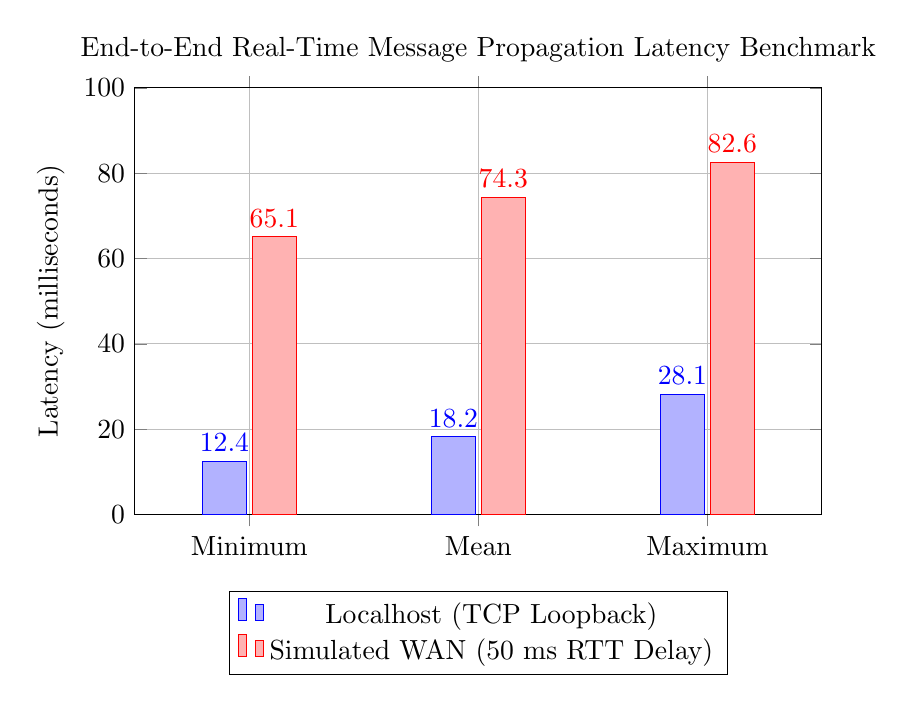
\begin{tikzpicture}
\begin{axis}[
    ybar,
    bar width=16pt,
    width=0.85\textwidth,
    height=7cm,
    ymin=0,
    ymax=100,
    enlarge x limits=0.25,
    ylabel={Latency (milliseconds)},
    symbolic x coords={Minimum,Mean,Maximum},
    xtick=data,
    nodes near coords,
    nodes near coords align={vertical},
    legend style={
        at={(0.5,-0.18)},
        anchor=north,
        legend columns=1
    },
    title={End-to-End Real-Time Message Propagation Latency Benchmark},
    grid=major
]

\addplot coordinates {
    (Minimum,12.4)
    (Mean,18.2)
    (Maximum,28.1)
};

\addplot coordinates {
    (Minimum,65.1)
    (Mean,74.3)
    (Maximum,82.6)
};

\legend{
    Localhost (TCP Loopback),
    Simulated WAN (50 ms RTT Delay)
}

\end{axis}
\end{tikzpicture}

\caption{Comparison of real-time message latency under Localhost and Simulated WAN network environments ($N=100$).}
\label{fig:latency_chart}
\end{figure}

The measured results satisfy the NFR-01 target of less than 100~ms under both tested network conditions. Mean delivery latency under local conditions was 18.2~ms ($\pm$ 3.4~ms), while the simulated WAN environment produced a mean latency of 74.3~ms ($\pm$ 4.1~ms).

The difference between the two environments is consistent with the additional network delay introduced in the simulated WAN configuration. Nevertheless, the maximum observed latency remained below the 100~ms NFR-01 threshold. These results indicate that the persistent real-time communication mechanism implemented using Socket.io provided responsive message delivery under the tested conditions.

\subsubsection{End-to-End Message Dispatch Process}

The end-to-end message transmission process was also examined to verify the interaction between the client applications, the Socket.io server, and persistent message storage.

\begin{figure}[htbp]
\centering

\resizebox{0.92\textwidth}{!}{%
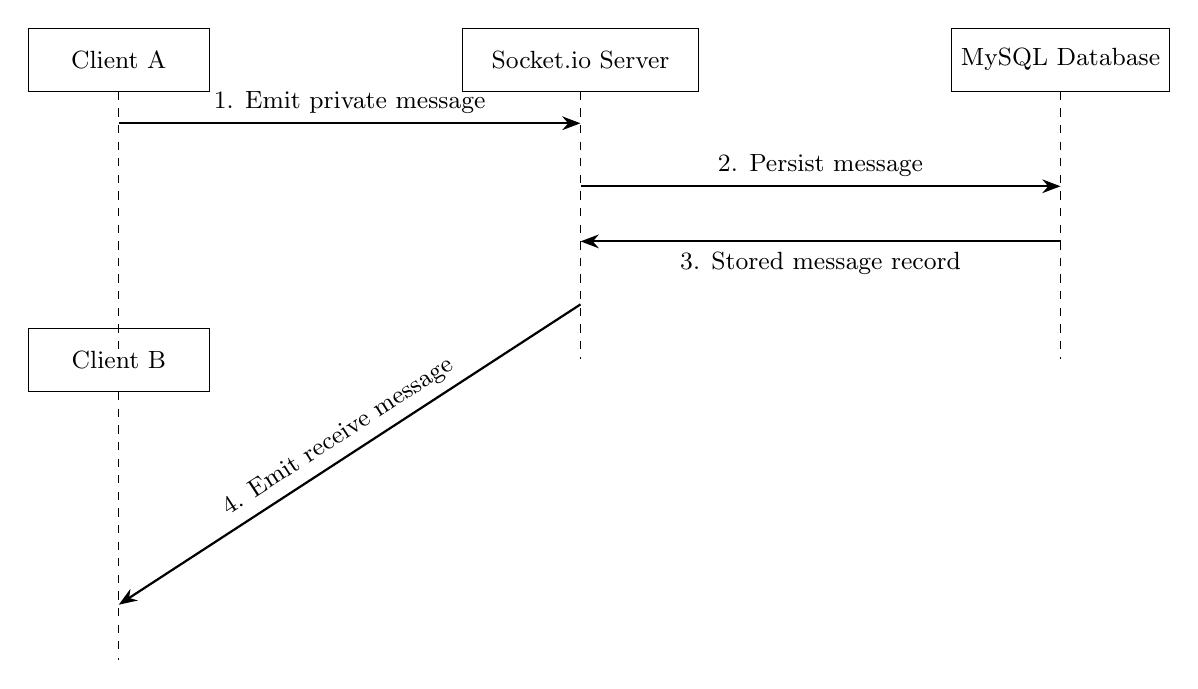
\begin{tikzpicture}[
    node distance=2.0cm,
    >=Stealth,
    font=\small,
    every node/.style={align=center}
]

% Nodes
\node[
    draw,
    rectangle,
    minimum width=2.3cm,
    minimum height=0.8cm
] (clientA) {Client A};

\node[
    draw,
    rectangle,
    minimum width=3.0cm,
    minimum height=0.8cm,
    right=3.2cm of clientA
] (server) {Socket.io Server};

\node[
    draw,
    rectangle,
    minimum width=2.3cm,
    minimum height=0.8cm,
    right=3.2cm of server
] (db) {MySQL Database};

\node[
    draw,
    rectangle,
    minimum width=2.3cm,
    minimum height=0.8cm,
    below=3.0cm of clientA
] (clientB) {Client B};

% Lifelines
\draw[dashed] (clientA.south) -- ++(0,-3.4);
\draw[dashed] (server.south) -- ++(0,-3.4);
\draw[dashed] (db.south) -- ++(0,-3.4);
\draw[dashed] (clientB.south) -- ++(0,-3.4);

% Message flow
\draw[->, thick]
    ($(clientA.south)+(0,-0.4)$)
    -- node[above] {1. Emit private message}
    ($(server.south)+(0,-0.4)$);

\draw[->, thick]
    ($(server.south)+(0,-1.2)$)
    -- node[above] {2. Persist message}
    ($(db.south)+(0,-1.2)$);

\draw[<-, thick]
    ($(server.south)+(0,-1.9)$)
    -- node[below] {3. Stored message record}
    ($(db.south)+(0,-1.9)$);

\draw[->, thick]
    ($(server.south)+(0,-2.7)$)
    -- node[above, sloped] {4. Emit receive message}
    ($(clientB.south)+(0,-2.7)$);

\end{tikzpicture}%
}

\caption{End-to-End Sequence Diagram of Real-Time Message Dispatch and Message Persistence.}
\label{fig:sequence_diagram}
\end{figure}

Figure~\ref{fig:sequence_diagram} illustrates the message transmission process implemented in Nextalk. When Client A sends a private message, the Socket.io server receives the event and processes the message. The message is then persisted before the corresponding real-time event is emitted to Client B.

This sequence separates real-time event delivery from persistent storage while maintaining a consistent message flow between the sender and recipient. The diagram therefore provides a functional representation of how Socket.io communication is integrated with the application's persistent data layer.

\subsubsection{Comparison with Existing Literature and Communication Protocols}

The observed system behaviour was comparatively considered against established web communication paradigms documented in networking literature.

\begin{itemize}

    \item
    \textbf{Comparison with HTTP Short Polling:}
    Short polling repeatedly sends HTTP requests to check whether new data is available. This approach may introduce repeated request and header overhead, particularly when no new event is available. In contrast, WebSocket communication maintains a persistent connection after the initial handshake and supports bidirectional communication through WebSocket frames \cite{rfc7230,rfc6455}.

    \item
    \textbf{Comparison with HTTP Long Polling:}
    Long polling keeps an HTTP request open until data becomes available or a timeout occurs, after which the client generally initiates another request. This repeated request cycle introduces additional communication overhead. Nextalk instead uses a persistent Socket.io connection for real-time event communication \cite{rfc6202}.

    \item
    \textbf{Comparison with Server-Sent Events (SSE):}
    Server-Sent Events provide a persistent mechanism for server-to-client event streaming. However, client-to-server communication normally requires separate HTTP requests. Nextalk uses Socket.io to provide bidirectional event communication through the same real-time communication mechanism.

\end{itemize}

The comparison indicates that the selected Socket.io architecture is appropriate for the interactive communication requirements of Nextalk, particularly for private messaging and real-time notification events.

\subsubsection{Critical Assessment of Own Work and System Limitations}

A critical assessment of the implemented system reveals several technical strengths and limitations.

\paragraph{Strengths}

\begin{enumerate}

    \item
    \textbf{Lightweight Frontend Architecture:}
    The frontend was implemented using Vite, TypeScript, HTML5, and CSS3 without relying on a large frontend framework. This resulted in a relatively lightweight client-side architecture while still supporting real-time messaging and social interaction interfaces.

    \item
    \textbf{Strict Type Safety:}
    TypeScript and Prisma provided compile-time type checking throughout the application. This reduced the likelihood of type-related errors during development and improved consistency between application logic and data models.

    \item
    \textbf{Real-Time Communication:}
    Socket.io provided a persistent communication mechanism for private messaging and real-time notification events. The latency evaluation demonstrated that the system remained below the NFR-01 target under both tested network conditions.

    \item
    \textbf{Privacy-Oriented User Discovery:}
    The use of a 6-digit \texttt{userCode} and UUID-based invite mechanism provided a convenient method for discovering users without requiring direct exposure of internal database identifiers.

\end{enumerate}

\paragraph{Limitations}

\begin{enumerate}

    \item
    \textbf{Single-Server Memory Constraint:}
    Active user socket sessions are maintained in an in-memory JavaScript \texttt{Map<number, string>}. Consequently, horizontal scaling across multiple application nodes is restricted because connection-state information is local to an individual server instance.

    \item
    \textbf{Uncompressed Media Storage:}
    Uploaded attachments are currently saved to disk in raw form without automated server-side compression, thumbnail generation, or CDN caching. This approach is suitable for the current prototype but may become inefficient as the number and size of uploaded files increase.

    \item
    \textbf{Limited Performance Evaluation Scope:}
    The latency evaluation was conducted using 100 consecutive message dispatches under two controlled network conditions. Although the results demonstrate compliance with the defined latency target under the tested conditions, they do not constitute a large-scale load test involving hundreds or thousands of concurrent users.

\end{enumerate}

\subsection{Discussion}

\subsubsection{Critical Analysis in Light of Scientific Literature}

The empirical findings support the suitability of persistent full-duplex communication for interactive web applications. WebSocket provides a communication channel that remains open after connection establishment and enables both the client and server to transmit messages without repeatedly initiating independent HTTP requests \cite{rfc6455}.

The measured mean latency of 18.2~ms under local TCP loopback conditions demonstrates that the application can provide highly responsive message delivery in a low-network-delay environment. Under the simulated WAN condition with an injected 50~ms RTT delay, the mean latency increased to 74.3~ms. The increase is expected because network propagation and transport delay contribute directly to end-to-end communication time.

Despite this increase, the maximum observed latency remained at 82.6~ms, which is below the NFR-01 threshold of 100~ms. Therefore, within the scope of the benchmark, the selected Socket.io communication architecture satisfied the defined real-time messaging requirement.

Furthermore, Node.js uses a non-blocking event-driven architecture based on the underlying \texttt{libuv} library. This programming model is suitable for applications that maintain many concurrent network connections because I/O operations can be handled asynchronously rather than requiring a dedicated thread for every active connection.

The results therefore suggest that the combination of Node.js and Socket.io is appropriate for the communication requirements of the Nextalk prototype.

\subsubsection{Analysis of System Limitations and Proposed Alternative Strategies}

The limitations identified during implementation provide several opportunities for future architectural improvement.

\paragraph{Horizontal Scaling via Redis Pub/Sub}

The current implementation maintains active socket-session mappings in application memory. While this approach is simple and effective for a single-server deployment, the mapping is not automatically shared between multiple application instances.

A scalable alternative is to introduce a Redis-based Socket.io adapter. The adapter can propagate events between multiple Node.js server instances, allowing users connected to different application instances to communicate through a shared messaging layer.

The proposed architecture is illustrated in Figure~\ref{fig:redis_architecture}.

\begin{figure}[htbp]
\centering

\resizebox{0.88\textwidth}{!}{%
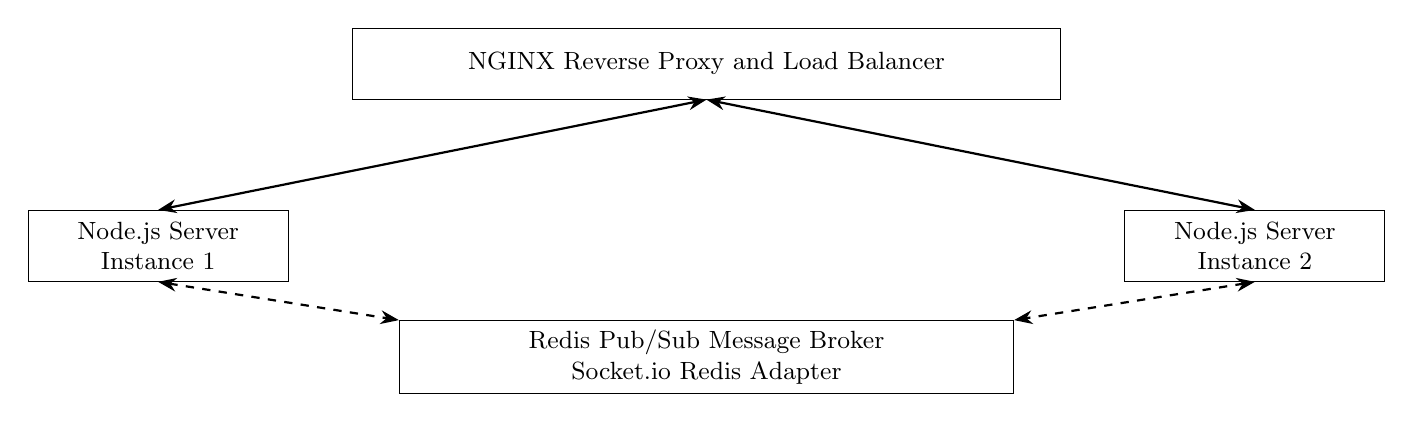
\begin{tikzpicture}[
    node distance=1.4cm,
    >=Stealth,
    font=\small,
    every node/.style={align=center}
]

% Load balancer
\node[
    draw,
    rectangle,
    minimum width=9.0cm,
    minimum height=0.9cm
] (lb) {NGINX Reverse Proxy and Load Balancer};

% Servers
\node[
    draw,
    rectangle,
    minimum width=3.3cm,
    minimum height=0.9cm,
    below left=1.4cm and 0.8cm of lb
] (server1) {Node.js Server\\Instance 1};

\node[
    draw,
    rectangle,
    minimum width=3.3cm,
    minimum height=0.9cm,
    below right=1.4cm and 0.8cm of lb
] (server2) {Node.js Server\\Instance 2};

% Redis
\node[
    draw,
    rectangle,
    minimum width=7.8cm,
    minimum height=0.9cm,
    below=2.8cm of lb
] (redis) {Redis Pub/Sub Message Broker\\
Socket.io Redis Adapter};

% Connections
\draw[<->, thick]
    (lb.south) -- (server1.north);

\draw[<->, thick]
    (lb.south) -- (server2.north);

\draw[<->, dashed, thick]
    (server1.south) -- (redis.north west);

\draw[<->, dashed, thick]
    (server2.south) -- (redis.north east);

\end{tikzpicture}%
}

\caption{Proposed Multi-Server Horizontal Scaling Architecture Using Redis Pub/Sub.}
\label{fig:redis_architecture}
\end{figure}

In this architecture, multiple Node.js server instances operate behind an NGINX reverse proxy and load balancer. Redis provides an intermediate communication layer that allows Socket.io events to be propagated between application instances.

This architecture removes the dependency on a single application's local socket-state mapping and provides a foundation for horizontal scaling. However, the additional infrastructure also increases deployment complexity and operational requirements.

\paragraph{Media Processing and Cloud Storage Pipeline}

The current media handling mechanism stores uploaded files directly on the application server. For a larger deployment, a dedicated media-processing pipeline could be introduced.

An image processing library such as \texttt{sharp} could be used to resize and compress uploaded images before storage. Object storage services such as Amazon S3 or Cloudflare R2 could then be used to separate media storage from the application servers.

This approach would reduce local disk dependency and provide a more scalable mechanism for handling large numbers of media files.

\subsubsection{Technical Contributions and Practical Significance}

This thesis provides several practical insights into the development of real-time full-stack web applications.

\begin{itemize}

    \item
    \textbf{Lightweight Real-Time Architecture:}
    The selected architecture, consisting of Vite, TypeScript, custom CSS, Node.js, Socket.io, and Prisma ORM, provides the required real-time communication and social interaction functionality without requiring a large frontend framework.

    \item
    \textbf{Demonstrated Real-Time Performance:}
    The latency benchmark demonstrated mean message delivery times of 18.2~ms under local TCP loopback conditions and 74.3~ms under the simulated WAN condition. Both results remained within the defined NFR-01 target of less than 100~ms.

    \item
    \textbf{Privacy-Oriented User Discovery Pattern:}
    The system uses unique 6-digit numerical identifiers (\texttt{userCode}) and UUID-based invite codes to provide user discovery while avoiding direct exposure of internal database primary keys.

    \item
    \textbf{Integrated Social and Communication Functions:}
    Nextalk combines private messaging, friendship management, media sharing, social posts, comments, likes, and notifications within a unified full-stack application architecture.

\end{itemize}

\subsubsection{Immediate Perspectives and Future Work Scope}

Building upon the achievements and limitations of Nextalk, several directions are proposed for future research and engineering development.

\begin{itemize}

    \item
    \textbf{End-to-End Encryption (E2EE):}
    Future versions could implement client-side message encryption using an established secure messaging protocol such as the Signal Protocol. This would provide stronger confidentiality by preventing plaintext message contents from being directly accessible to the server-side application layer.

    \item
    \textbf{WebRTC Audio/Video Calling:}
    Socket.io signaling could be extended to support WebRTC-based peer-to-peer audio and video communication. In such an architecture, Socket.io would primarily coordinate session establishment while WebRTC would handle real-time media transmission.

    \item
    \textbf{Horizontal Server Scaling:}
    The proposed Redis Pub/Sub architecture could be implemented to allow multiple Node.js instances to operate behind a load balancer. Future experiments could evaluate the resulting system under increasing numbers of concurrent connections.

    \item
    \textbf{Media Optimization and Cloud Storage:}
    The media subsystem could be enhanced through automatic image compression, thumbnail generation, WebP conversion, and object storage integration.

    \item
    \textbf{Containerization and Deployment Automation:}
    Docker could be introduced to standardize the deployment of the backend, frontend, database, and supporting services. Kubernetes could subsequently be considered for automated orchestration and horizontal scaling in larger production environments.

    \item
    \textbf{Large-Scale Performance Evaluation:}
    Future work should include controlled load testing with increasing numbers of concurrent users and message events. Such experiments would provide a more comprehensive evaluation of throughput, latency distribution, resource utilization, and system scalability.

\end{itemize}

\newpage
% ==============================================================================
% V/ CONCLUSION & PERSPECTIVE
% ==============================================================================

\section{CONCLUSION \& PERSPECTIVE}

\subsection{Conclusion}

This thesis presented the design, implementation, and evaluation of
\textbf{Nextalk}, a lightweight web-based real-time chat and social
interaction system. The system integrates private real-time messaging,
typing indicators, message persistence, user authentication, user
discovery, friendship management, posts, likes, nested comments, and
real-time notifications.

The functional evaluation confirmed the successful operation of the
implemented core features. In addition, the real-time communication
evaluation achieved the defined latency target of less than 100~ms under
the tested local and simulated WAN conditions. These results demonstrate
that the proposed architecture can effectively support the main
requirements of a real-time chat and social interaction platform.

However, the current system remains primarily designed for a
single-server environment, with local media storage and limited support
for advanced real-time communication features. These limitations provide
clear opportunities for further development.

\subsection{Perspective}

Future development of \textbf{Nextalk} could focus on improving
scalability, security, and communication capabilities. WebRTC could be
integrated to support real-time audio and video calling, while Socket.io
rooms could be extended to provide group chats and channels.

For larger-scale deployment, a distributed Socket.io architecture using
Redis or another shared message broker could be introduced. Cloud-based
object storage, image compression, and CDN delivery could also replace
the current local media storage approach. Finally, an appropriate
end-to-end encryption mechanism could be investigated to improve the
confidentiality of private communications.

% ==============================================================================
% REFERENCES
% ==============================================================================

\newpage

\section*{REFERENCES}
\addcontentsline{toc}{section}{REFERENCES}

\begin{thebibliography}{99}

\bibitem{rfc7230}
R. Fielding and J. Reschke,
``Hypertext Transfer Protocol (HTTP/1.1): Message Syntax and Routing,''
IETF RFC 7230, June 2014.
[Online]. Available: \url{https://www.rfc-editor.org/rfc/rfc7230}

\bibitem{rfc6202}
S. Loreto, P. Saint-Andre, S. Salsano, and G. Wilkins,
``Known Issues and Best Practices for the Use of Long Polling and Streaming
in Bidirectional HTTP,''
IETF RFC 6202, Apr. 2011.
[Online]. Available: \url{https://www.rfc-editor.org/rfc/rfc6202}

\bibitem{w3c_sse}
I. Hickson, ed.,
``Server-Sent Events,''
W3C Recommendation, Feb. 3, 2015.
[Online]. Available: \url{https://www.w3.org/TR/eventsource/}

\bibitem{rfc6455}
I. Fette and A. Melnikov,
``The WebSocket Protocol,''
IETF RFC 6455, Dec. 2011.
[Online]. Available: \url{https://www.rfc-editor.org/rfc/rfc6455}

\bibitem{nodejs_patterns}
M. Cantelon, M. Harter, T. J. Holowaychuk, and N. Rajlich,
\textit{Node.js in Action}.
Shelter Island, NY, USA: Manning Publications, 2014.

\bibitem{typescript_doc}
Microsoft,
``TypeScript Documentation.''
[Online]. Available: \url{https://www.typescriptlang.org/docs/}

\bibitem{socketio_doc}
Socket.IO,
``Socket.IO Documentation: Bidirectional and Event-Based Communication.''
[Online]. Available: \url{https://socket.io/docs/v4/}

\bibitem{prisma_doc}
Prisma,
``Prisma Documentation.''
[Online]. Available: \url{https://www.prisma.io/docs}

\bibitem{rfc7519}
M. Jones, J. Bradley, and N. Sakimura,
``JSON Web Token (JWT),''
IETF RFC 7519, May 2015.
[Online]. Available: \url{https://www.rfc-editor.org/rfc/rfc7519}

\bibitem{bcrypt_paper}
N. Provos and D. Mazi\`eres,
``A Future-Adaptable Password Scheme,''
in \textit{Proceedings of the 1999 USENIX Annual Technical Conference
(USENIX ATC 99)}, Monterey, CA, USA, 1999, pp. 81--92.
[Online]. Available:
\url{https://www.usenix.org/conference/1999-usenix-annual-technical-conference/future-adaptable-password-scheme}

\bibitem{express_doc}
Express.js,
``Express -- Fast, Unopinionated, Minimalist Web Framework for Node.js.''
[Online]. Available: \url{https://expressjs.com/}

\end{thebibliography}

% ==============================================================================
% APPENDICES
% ==============================================================================

\newpage

\appendix

\section{PROJECT WEBSITE}

The official website of the Nextalk system is available at:

\begin{center}
    \url{https://nextalk.pro.vn}
\end{center}

% ==============================================================================
% DOCUMENT END
% ==============================================================================

\end{document}
